\documentclass[12pt,twoside]{article}

\usepackage{amsmath}
\usepackage{color}
\usepackage{enumitem}
\usepackage{graphicx}
\graphicspath{ {images/} }

\usepackage{subfig}
\usepackage{placeins}
\usepackage{float}


\usepackage{mdframed}


\newcommand{\cross}[1][1pt]{\ooalign{%
  \rule[1ex]{1ex}{#1}\cr% Horizontal bar
  \hss\rule{#1}{.7em}\hss\cr}}% Vertical bar

% Cross-references for handout numbers.

\newcommand{\name}{}

\usepackage{latexsym}
%\usepackage{bbm}
\usepackage{times,url}
\usepackage{clrscode}

\newcommand{\mitst}[1]{\begin{description}
\item[MIT students:] #1
\end{description}}
\newcommand{\smast}[1]{\begin{description}
\item[SMA students:] #1
\end{description}}

\newcommand{\profs}{Professor Chris Rycroft}
\newcommand{\subj}{AM205}

\newlength{\toppush}
\setlength{\toppush}{2\headheight}
\addtolength{\toppush}{\headsep}

\newcommand{\htitle}[2]{\noindent\vspace*{-\toppush}\newline\parbox{6.5in}
{\textit{Advanced Scientific Computing: Numerical Methods AM205}\hfill\name\newline
Harvard University \hfill #2\newline
\profs\hfill #1 \vspace*{-.5ex}\newline
\mbox{}\hrulefill\mbox{}}\vspace*{1ex}\mbox{}\newline
\begin{center}{\Large\bf #1}\end{center}}

\newcommand{\handout}[2]{\thispagestyle{empty}
 \markboth{#1}{#1}
 \pagestyle{myheadings}\htitle{#1}{#2}}

\newcommand{\htitlewithouttitle}[2]{\noindent\vspace*{-\toppush}\newline\parbox{6.5in}
{\textit{Introduction to Algorithms}\hfill#2\newline
Massachusetts Institute of Technology \hfill 6.006\newline
%Singapore-MIT Alliance \hfill SMA5503\newline
\profs\hfill Handout #1\vspace*{-.5ex}\newline
\mbox{}\hrulefill\mbox{}}\vspace*{1ex}\mbox{}\newline}

\newcommand{\handoutwithouttitle}[2]{\thispagestyle{empty}
 \markboth{Handout \protect\ref{#1}}{Handout \protect\ref{#1}}
 \pagestyle{myheadings}\htitlewithouttitle{\protect\ref{#1}}{#2}}

\newcommand{\exam}[2]{% parameters: exam name, date
 \thispagestyle{empty}
 \markboth{\subj\ #1\hspace{1in}Name\hrulefill\ \ }%
          {\subj\ #1\hspace{1in}Name\hrulefill\ \ }
 \pagestyle{myheadings}\examtitle{#1}{#2}
 \renewcommand{\theproblem}{Problem \arabic{problemnum}}
}
\newcommand{\examsolutions}[3]{% parameters: handout, exam name, date
 \thispagestyle{empty}
 \markboth{Handout \protect\ref{#1}: #2}{Handout \protect\ref{#1}: #2}
% \pagestyle{myheadings}\htitle{\protect\ref{#1}}{#2}{#3}
 \pagestyle{myheadings}\examsolutionstitle{\protect\ref{#1}} {#2}{#3}
 \renewcommand{\theproblem}{Problem \arabic{problemnum}}
}
\newcommand{\examsolutionstitle}[3]{\noindent\vspace*{-\toppush}\newline\parbox{6.5in}
{\textit{Introduction to Algorithms}\hfill#3\newline
Massachusetts Institute of Technology \hfill 6.006\newline
%Singapore-MIT Alliance \hfill SMA5503\newline
\profs\hfill Handout #1\vspace*{-.5ex}\newline
\mbox{}\hrulefill\mbox{}}\vspace*{1ex}\mbox{}\newline
\begin{center}{\Large\bf #2}\end{center}}

\newcommand{\takehomeexam}[2]{% parameters: exam name, date
 \thispagestyle{empty}
 \markboth{\subj\ #1\hfill}{\subj\ #1\hfill}
 \pagestyle{myheadings}\examtitle{#1}{#2}
 \renewcommand{\theproblem}{Problem \arabic{problemnum}}
}

\makeatletter
\newcommand{\exambooklet}[2]{% parameters: exam name, date
 \thispagestyle{empty}
 \markboth{\subj\ #1}{\subj\ #1}
 \pagestyle{myheadings}\examtitle{#1}{#2}
 \renewcommand{\theproblem}{Problem \arabic{problemnum}}
 \renewcommand{\problem}{\newpage
 \item \let\@currentlabel=\theproblem
 \markboth{\subj\ #1, \theproblem}{\subj\ #1, \theproblem}}
}
\makeatother


\newcommand{\examtitle}[2]{\noindent\vspace*{-\toppush}\newline\parbox{6.5in}
{\textit{Advanced Scientific Computing: Numerical Methods}\hfill#2\newline
Harvard University \hfill AM205 Fall 2017\newline
%Singapore-MIT Alliance \hfill SMA5503\newline
\profs\hfill #1\vspace*{-.5ex}\newline
\mbox{}\hrulefill\mbox{}}\vspace*{1ex}\mbox{}\newline
\begin{center}{\Large\bf #1}\end{center}}

\newcommand{\grader}[1]{\hspace{1cm}\textsf{\textbf{#1}}\hspace{1cm}}

\newcommand{\points}[1]{[#1 points]\ }
\newcommand{\parts}[1]
{
  \ifnum#1=1
  (1 part)
  \else
  (#1 parts)
  \fi
  \
}

\newcommand{\bparts}{\begin{problemparts}}
\newcommand{\eparts}{\end{problemparts}}
\newcommand{\ppart}{\problempart}

%\newcommand{\lg} {lg\ }

\setlength{\oddsidemargin}{0pt}
\setlength{\evensidemargin}{0pt}
\setlength{\textwidth}{6.5in}
\setlength{\topmargin}{0in}
\setlength{\textheight}{8.5in}


\newcommand{\Spawn}{{\bf spawn} }
\newcommand{\Sync}{{\bf sync}}

\renewcommand{\cases}[1]{\left\{ \begin{array}{ll}#1\end{array}\right.}
\newcommand{\cif}[1]{\mbox{if $#1$}}
\newcommand{\cwhen}[1]{\mbox{when $#1$}}

\newcounter{problemnum}
\newcommand{\theproblem}{Problem \theproblemsetnum-\arabic{problemnum}}
\newenvironment{problems}{
        \begin{list}{{\bf \theproblem. \hspace*{0.5em}}}
        {\setlength{\leftmargin}{0em}
         \setlength{\rightmargin}{0em}
         \setlength{\labelwidth}{0em}
         \setlength{\labelsep}{0em}
         \usecounter{problemnum}}}{\end{list}}
\makeatletter
\newcommand{\problem}[1][{}]{\item \let\@currentlabel=\theproblem \textbf{#1}}
\makeatother

\newcounter{problempartnum}[problemnum]
\newenvironment{problemparts}{
        \begin{list}{{\bf (\alph{problempartnum})}}
        {\setlength{\leftmargin}{2.5em}
         \setlength{\rightmargin}{2.5em}
         \setlength{\labelsep}{0.5em}}}{\end{list}}
\newcommand{\problempart}{\addtocounter{problempartnum}{1}\item}

\newenvironment{truefalseproblemparts}{
        \begin{list}{{\bf (\alph{problempartnum})\ \ \ T\ \ F\hfil}}
        {\setlength{\leftmargin}{4.5em}
         \setlength{\rightmargin}{2.5em}
         \setlength{\labelsep}{0.5em}
         \setlength{\labelwidth}{4.5em}}}{\end{list}}

\newcounter{exercisenum}
\newcommand{\theexercise}{Exercise \theproblemsetnum-\arabic{exercisenum}}
\newenvironment{exercises}{
        \begin{list}{{\bf \theexercise. \hspace*{0.5em}}}
        {\setlength{\leftmargin}{0em}
         \setlength{\rightmargin}{0em}
         \setlength{\labelwidth}{0em}
         \setlength{\labelsep}{0em}
        \usecounter{exercisenum}}}{\end{list}}
\makeatletter
\newcommand{\exercise}{\item \let\@currentlabel=\theexercise}
\makeatother

\newcounter{exercisepartnum}[exercisenum]
%\newcommand{\problem}[1]{\medskip\mbox{}\newline\noindent{\bf Problem #1.}\hspace*{1em}}
%\newcommand{\exercise}[1]{\medskip\mbox{}\newline\noindent{\bf Exercise #1.}\hspace*{1em}}

\newenvironment{exerciseparts}{
        \begin{list}{{\bf (\alph{exercisepartnum})}}
        {\setlength{\leftmargin}{2.5em}
         \setlength{\rightmargin}{2.5em}
         \setlength{\labelsep}{0.5em}}}{\end{list}}
\newcommand{\exercisepart}{\addtocounter{exercisepartnum}{1}\item}


% Macros to make captions print with small type and 'Figure xx' in bold.
\makeatletter
\def\fnum@figure{{\bf Figure \thefigure}}
\def\fnum@table{{\bf Table \thetable}}
\let\@mycaption\caption
%\long\def\@mycaption#1[#2]#3{\addcontentsline{\csname
%  ext@#1\endcsname}{#1}{\protect\numberline{\csname
%  the#1\endcsname}{\ignorespaces #2}}\par
%  \begingroup
%    \@parboxrestore
%    \small
%    \@makecaption{\csname fnum@#1\endcsname}{\ignorespaces #3}\par
%  \endgroup}
%\def\mycaption{\refstepcounter\@captype \@dblarg{\@mycaption\@captype}}
%\makeatother
\let\mycaption\caption
%\newcommand{\figcaption}[1]{\mycaption[]{#1}}

\newcounter{totalcaptions}
\newcounter{totalart}

\newcommand{\figcaption}[1]{\addtocounter{totalcaptions}{1}\caption[]{#1}}

% \psfigures determines what to do for figures:
%       0 means just leave vertical space
%       1 means put a vertical rule and the figure name
%       2 means insert the PostScript version of the figure
%       3 means put the figure name flush left or right
\newcommand{\psfigures}{0}
\newcommand{\spacefigures}{\renewcommand{\psfigures}{0}}
\newcommand{\rulefigures}{\renewcommand{\psfigures}{1}}
\newcommand{\macfigures}{\renewcommand{\psfigures}{2}}
\newcommand{\namefigures}{\renewcommand{\psfigures}{3}}

\newcommand{\figpart}[1]{{\bf (#1)}\nolinebreak[2]\relax}
\newcommand{\figparts}[2]{{\bf (#1)--(#2)}\nolinebreak[2]\relax}


\macfigures     % STATE

% When calling \figspace, make sure to leave a blank line afterward!!
% \widefigspace is for figures that are more than 28pc wide.
\newlength{\halffigspace} \newlength{\wholefigspace}
\newlength{\figruleheight} \newlength{\figgap}
\newcommand{\setfiglengths}{\ifnum\psfigures=1\setlength{\figruleheight}{\hruleheight}\setlength{\figgap}{1em}\else\setlength{\figruleheight}{0pt}\setlength{\figgap}{0em}\fi}
\newcommand{\figspace}[2]{\ifnum\psfigures=0\leavefigspace{#1}\else%
\setfiglengths%
\setlength{\wholefigspace}{#1}\setlength{\halffigspace}{.5\wholefigspace}%
\rule[-\halffigspace]{\figruleheight}{\wholefigspace}\hspace{\figgap}#2\fi}
\newlength{\widefigspacewidth}
% Make \widefigspace put the figure flush right on the text page.
\newcommand{\widefigspace}[2]{
\ifnum\psfigures=0\leavefigspace{#1}\else%
\setfiglengths%
\setlength{\widefigspacewidth}{28pc}%
\addtolength{\widefigspacewidth}{-\figruleheight}%
\setlength{\wholefigspace}{#1}\setlength{\halffigspace}{.5\wholefigspace}%
\makebox[\widefigspacewidth][r]{#2\hspace{\figgap}}\rule[-\halffigspace]{\figruleheight}{\wholefigspace}\fi}
\newcommand{\leavefigspace}[1]{\setlength{\wholefigspace}{#1}\setlength{\halffigspace}{.5\wholefigspace}\rule[-\halffigspace]{0em}{\wholefigspace}}

% Commands for including figures with macpsfig.
% To use these commands, documentstyle ``macpsfig'' must be specified.
\newlength{\macfigfill}
\makeatother
\newlength{\bbx}
\newlength{\bby}
\newcommand{\macfigure}[5]{\addtocounter{totalart}{1}
\ifnum\psfigures=2%
\setlength{\bbx}{#2}\addtolength{\bbx}{#4}%
\setlength{\bby}{#3}\addtolength{\bby}{#5}%
\begin{flushleft}
\ifdim#4>28pc\setlength{\macfigfill}{#4}\addtolength{\macfigfill}{-28pc}\hspace*{-\macfigfill}\fi%
\mbox{\psfig{figure=./#1.ps,%
bbllx=#2,bblly=#3,bburx=\bbx,bbury=\bby}}
\end{flushleft}%
\else\ifdim#4>28pc\widefigspace{#5}{#1}\else\figspace{#5}{#1}\fi\fi}
\makeatletter

\newlength{\savearraycolsep}
\newcommand{\narrowarray}[1]{\setlength{\savearraycolsep}{\arraycolsep}\setlength{\arraycolsep}{#1\arraycolsep}}
\newcommand{\normalarray}{\setlength{\arraycolsep}{\savearraycolsep}}

\newcommand{\hint}{{\em Hint:\ }}

% Macros from /th/u/clr/mac.tex

\newcommand{\set}[1]{\left\{ #1 \right\}}
\newcommand{\abs}[1]{\left| #1\right|}
\newcommand{\card}[1]{\left| #1\right|}
\newcommand{\floor}[1]{\left\lfloor #1 \right\rfloor}
\newcommand{\ceil}[1]{\left\lceil #1 \right\rceil}
\newcommand{\ang}[1]{\ifmmode{\left\langle #1 \right\rangle}
   \else{$\left\langle${#1}$\right\rangle$}\fi}
        % the \if allows use outside mathmode,
        % but will swallow following space there!
\newcommand{\paren}[1]{\left( #1 \right)}
\newcommand{\bracket}[1]{\left[ #1 \right]}
\newcommand{\prob}[1]{\Pr\left\{ #1 \right\}}
\newcommand{\Var}{\mathop{\rm Var}\nolimits}
\newcommand{\expect}[1]{{\rm E}\left[ #1 \right]}
\newcommand{\expectsq}[1]{{\rm E}^2\left[ #1 \right]}
\newcommand{\variance}[1]{{\rm Var}\left[ #1 \right]}
\renewcommand{\choose}[2]{{{#1}\atopwithdelims(){#2}}}
\def\pmod#1{\allowbreak\mkern12mu({\rm mod}\,\,#1)}
\newcommand{\matx}[2]{\left(\begin{array}{*{#1}{c}}#2\end{array}\right)}
\newcommand{\Adj}{\mathop{\rm Adj}\nolimits}

\newtheorem{theorem}{Theorem}
\newtheorem{lemma}[theorem]{Lemma}
\newtheorem{corollary}[theorem]{Corollary}
\newtheorem{xample}{Example}
\newtheorem{definition}{Definition}
\newenvironment{example}{\begin{xample}\rm}{\end{xample}}
\newcommand{\proof}{\noindent{\em Proof.}\hspace{1em}}
\def\squarebox#1{\hbox to #1{\hfill\vbox to #1{\vfill}}}
\newcommand{\qedbox}{\vbox{\hrule\hbox{\vrule\squarebox{.667em}\vrule}\hrule}}
\newcommand{\qed}{\nopagebreak\mbox{}\hfill\qedbox\smallskip}
\newcommand{\eqnref}[1]{(\protect\ref{#1})}

%%\newcommand{\twodots}{\mathinner{\ldotp\ldotp}}
\newcommand{\transpose}{^{\mbox{\scriptsize \sf T}}}
\newcommand{\amortized}[1]{\widehat{#1}}

\newcommand{\punt}[1]{}

%%% command for putting definitions into boldface
% New style for defined terms, as of 2/23/88, redefined by THC.
\newcommand{\defn}[1]{{\boldmath\textit{\textbf{#1}}}}
\newcommand{\defi}[1]{{\textit{\textbf{#1\/}}}}

\newcommand{\red}{\leq_{\rm P}}
\newcommand{\lang}[1]{%
\ifmmode\mathord{\mathcode`-="702D\rm#1\mathcode`\-="2200}\else{\rm#1}\fi}

%\newcommand{\ckt}[1]{\ifmmode\mathord{\mathcode`-="702D\sc #1\mathcode`\-="2200}\else$\mathord{\mathcode`-="702D\sc #1\mathcode`\-="2200}$\fi}
\newcommand{\ckt}[1]{\ifmmode \sc #1\else$\sc #1$\fi}

%% Margin notes - use \notesfalse to turn off notes.
\setlength{\marginparwidth}{0.6in}
\reversemarginpar
\newif\ifnotes
\notestrue
\newcommand{\longnote}[1]{
  \ifnotes
    {\medskip\noindent Note: \marginpar[\hfill$\Longrightarrow$]
      {$\Longleftarrow$}{#1}\medskip}
  \fi}
\newcommand{\note}[1]{
  \ifnotes
    {\marginpar{\tiny \raggedright{#1}}}
  \fi}


\newcommand{\reals}{\mathbbm{R}}
\newcommand{\integers}{\mathbbm{Z}}
\newcommand{\naturals}{\mathbbm{N}}
\newcommand{\rationals}{\mathbbm{Q}}
\newcommand{\complex}{\mathbbm{C}}

\newcommand{\oldreals}{{\bf R}}
\newcommand{\oldintegers}{{\bf Z}}
\newcommand{\oldnaturals}{{\bf N}}
\newcommand{\oldrationals}{{\bf Q}}
\newcommand{\oldcomplex}{{\bf C}}

\newcommand{\w}{\omega}                 %% for fft chapter

\newenvironment{closeitemize}{\begin{list}
{$\bullet$}
{\setlength{\itemsep}{-0.2\baselineskip}
\setlength{\topsep}{0.2\baselineskip}
\setlength{\parskip}{0pt}}}
{\end{list}}

% These are necessary within a {problems} environment in order to restore
% the default separation between bullets and items.
\newenvironment{normalitemize}{\setlength{\labelsep}{0.5em}\begin{itemize}}
                              {\end{itemize}}
\newenvironment{normalenumerate}{\setlength{\labelsep}{0.5em}\begin{enumerate}}
                                {\end{enumerate}}

%\def\eqref#1{Equation~(\ref{eq:#1})}
%\newcommand{\eqref}[1]{Equation (\ref{eq:#1})}
\newcommand{\eqreftwo}[2]{Equations (\ref{eq:#1}) and~(\ref{eq:#2})}
\newcommand{\ineqref}[1]{Inequality~(\ref{ineq:#1})}
\newcommand{\ineqreftwo}[2]{Inequalities (\ref{ineq:#1}) and~(\ref{ineq:#2})}

\newcommand{\figref}[1]{Figure~\ref{fig:#1}}
\newcommand{\figreftwo}[2]{Figures \ref{fig:#1} and~\ref{fig:#2}}

\newcommand{\liref}[1]{line~\ref{li:#1}}
\newcommand{\Liref}[1]{Line~\ref{li:#1}}
\newcommand{\lirefs}[2]{lines \ref{li:#1}--\ref{li:#2}}
\newcommand{\Lirefs}[2]{Lines \ref{li:#1}--\ref{li:#2}}
\newcommand{\lireftwo}[2]{lines \ref{li:#1} and~\ref{li:#2}}
\newcommand{\lirefthree}[3]{lines \ref{li:#1}, \ref{li:#2}, and~\ref{li:#3}}

\newcommand{\lemlabel}[1]{\label{lem:#1}}
\newcommand{\lemref}[1]{Lemma~\ref{lem:#1}}

\newcommand{\exref}[1]{Exercise~\ref{ex:#1}}

\newcommand{\handref}[1]{Handout~\ref{#1}}

\newcommand{\defref}[1]{Definition~\ref{def:#1}}

% (1997.8.16: Victor Luchangco)
% Modified \hlabel to only get date and to use handouts counter for number.
%   New \handout and \handoutwithouttitle commands in newmac.tex use this.
%   The date is referenced by <label>-date.
%   (Retained old definition as \hlabelold.)
%   Defined \hforcelabel to use an argument instead of the handouts counter.

\newcounter{handouts}
\setcounter{handouts}{0}

\newcommand{\hlabel}[2]{%
\stepcounter{handouts}
{\edef\next{\write\@auxout{\string\newlabel{#1}{{\arabic{handouts}}{0}}}}\next}
\write\@auxout{\string\newlabel{#1-date}{{#2}{0}}}
}

\newcommand{\hforcelabel}[3]{%          Does not step handouts counter.
\write\@auxout{\string\newlabel{#1}{{#2}{0}}}
\write\@auxout{\string\newlabel{#1-date}{{#3}{0}}}}


% less ugly underscore
% --juang, 2008 oct 05
\renewcommand{\_}{\vrule height 0 pt depth 0.4 pt width 0.5 em \,}



\setlength{\oddsidemargin}{0pt}
\setlength{\evensidemargin}{0pt}
\setlength{\textwidth}{6.5in}
\setlength{\topmargin}{0in}
\setlength{\textheight}{8.5in}

\newcommand{\theproblemsetnum}{}
\newcommand{\releasedate}{December 1, 2017}
\newcommand{\duedate}{December 1, 2017}
\newcommand{\tabUnit}{3ex}
\newcommand{\tabT}{\hspace*{\tabUnit}}

\usepackage{listings}
\usepackage{color}
\usepackage{amsmath}


\definecolor{dkgreen}{rgb}{0,0.6,0}
\definecolor{gray}{rgb}{0.5,0.5,0.5}
\definecolor{mauve}{rgb}{0.58,0,0.82}

\lstset{frame=tb,
  language=Python,
  aboveskip=3mm,
  belowskip=3mm,
  showstringspaces=false,
  columns=flexible,
  basicstyle={\small\ttfamily},
  numbers=none,
  numberstyle=\tiny\color{gray},
  keywordstyle=\color{blue},
  commentstyle=\color{dkgreen},
  stringstyle=\color{mauve},
  breaklines=true,
  breakatwhitespace=true,
  tabsize=3
}

\newcommand{\dd}[1]{\mathrm{d}#1}

\title{6.006 Problem Set 4}

\begin{document}

\handout{Crypto project \theproblemsetnum}{\releasedate} %{April 6, 2017}

\setlength{\parindent}{0pt}

\medskip

\hrulefill

\medskip

{\bf Name:} Yihang Yan, Tomas Gudmundsson, Nathaniel Stein

\medskip

\hrulefill

%%%%%%%%%%%%%%%%%%%%%%%%%%%%%%%%%%%%%%%%%%%%%%%%%%%%%
% See below for common and useful latex constructs. %
%%%%%%%%%%%%%%%%%%%%%%%%%%%%%%%%%%%%%%%%%%%%%%%%%%%%%

% Some useful commands:
%$f(x) = \Theta(x)$
%$T(x, y) \leq \log(x) + 2^y + \binom{2n}{n}$
% {\tt code\_function}


% You can create unnumbered lists as follows:
%\begin{itemize}
%    \item First item in a list 
%        \begin{itemize}
%            \item First item in a list 
%                \begin{itemize}
%                    \item First item in a list 
%                    \item Second item in a list 
%                \end{itemize}
%            \item Second item in a list 
%        \end{itemize}
%    \item Second item in a list 
%\end{itemize}

% You can create numbered lists as follows:
%\begin{enumerate}
%    \item First item in a list 
%    \item Second item in a list 
%    \item Third item in a list
%\end{enumerate}

% You can write aligned equations as follows:
%\begin{align} 
%    \begin{split}
%        (x+y)^3 &= (x+y)^2(x+y) \\
%                &= (x^2+2xy+y^2)(x+y) \\
%                &= (x^3+2x^2y+xy^2) + (x^2y+2xy^2+y^3) \\
%                &= x^3+3x^2y+3xy^2+y^3
%    \end{split}                                 
%\end{align}

% You can create grids/matrices as follows:
%\begin{align}
%    A = 
%    \begin{bmatrix}
%        A_{11} & A_{21} \\
%        A_{21} & A_{22}
%    \end{bmatrix}
%\end{align}
% http://www.aip.de/groups/soe/local/numres/bookcpdf/c11-1.pdf
\section*{1}
\subsection*{Jacobi method}
In order to find eigenvalues and eigenvectors of the covariance matrix, A, we use the Jacobi method. The method works by finding the largest non-diagonal element at location $(i,j)$ and makes it zero by doing a plane rotation on rows and columns $i$ and $j$. The Jacobi method is quite efficient with quadratic convergence and can be parallelized easily.  \\


The rotation for matrix A works as follows:
\begin{equation}
     A' = P_{i,j,\theta}^T \cdot A \cdot P_{i,j,\theta}  
\end{equation}

where $P_{i,j,\theta} = P(i,j,\theta)$ is a Givens rotation matrix with the form:

\begin{equation}
P(i,j,\theta) = 
\begin{bmatrix}
     1 & \cdots & 0 & \cdots & 0 & \cdots & 0 \\
     \vdots & \ddots & \vdots &   & \vdots &  & \vdots \\
          0 & \cdots & c & \cdots & s & \cdots & 0 \\
         \vdots &  & \vdots & \ddots  & \vdots &  & \vdots \\
     0 & \cdots & -s & \cdots & c & \cdots & 0 \\
              \vdots &  & \vdots &  & \vdots & \ddots  & \vdots \\
                   0 & \cdots & 0 & \cdots & 0 & \cdots & 1 \\
\end{bmatrix}
\end{equation}\\

This matrix has ones on the diagonal except where $c=cos(\theta)$ at locations (i,i) and (j,j). All other elements are 0 except $s=sin(\theta)$ at locations (i,j) and (j,i).\\

When the Givens rotation matrix, $P_{i,j,\theta}$,  is multiplied with another matrix, $A$, as $P\cdot A$ it simulates a clockwise rotation in the plane by an angle $\theta$ in order to nullify the element at location $(i,j)$ and only affects rows and columns $i$ and $j$ in the process.\\
 

In order to figure out the values of $c,s$ and $\theta$ we will simulate a matrix multiplication with $2x2$ matrices that contain the relevant information. We will represent the matrices as follows:
\begin{equation}
P_{i,j,\theta} = 
\begin{bmatrix}
     c_{ii} & s_{ij} \\
    -s_{ji} & c_{jj} \\
\end{bmatrix}
,A = 
\begin{bmatrix}
     A_{ii} & A_{ij} \\
    A_{ji} & A_{jj} \\
\end{bmatrix}
,A' = 
\begin{bmatrix}
     A_{ii}' & A_{ij}' \\
    A_{ji}' & A_{jj}' \\
\end{bmatrix}
\end{equation}

where the notation $A_{ij}$ denotes element at location $(i,j)$ in matrix A.\\


Now we will find $c, s$ and $\theta$ so that the matrix multiplication nullifies the largest element. In order for P to satisfy eq. 1 we expand the matrix multiplication as follows with $c_{ii}=c_{jj}=c$ and $s_{ji}=s_{ij}=s$:\\
\begin{equation}
\begin{split}
\begin{bmatrix}
     A_{ii}' & A_{ij}' \\
    A_{ji}' & A_{jj}' \\
\end{bmatrix}
 &=
\begin{bmatrix}
     c & -s \\
    s & c \\
\end{bmatrix}
\cdot
\begin{bmatrix}
     A_{ii} & A_{ij} \\
    A_{ji} & A_{jj} \\
\end{bmatrix}
\cdot
\begin{bmatrix}
     c & s \\
     -s & c \\
\end{bmatrix}\\
&=\begin{bmatrix}
     c\cdot A_{ii} - s\cdot A_{ji} & c\cdot A_{ij} - s\cdot A_{jj} \\
     s\cdot A_{ii} + c\cdot A_{ji} & s\cdot A_{ij} + c\cdot A_{jj} \\
\end{bmatrix}
\cdot
\begin{bmatrix}
     c & s \\
     -s & c \\
\end{bmatrix}\\
&=\begin{bmatrix}
c^2\cdot A_{ii} - cs\cdot A_{ji} - cs\cdot A_{ij} + s^2\cdot A_{jj} & cs\cdot A_{ii} - s^2\cdot A_{ji} + c^2\cdot A_{ij} - cs\cdot A_{jj}\\
cs\cdot A_{ii} + c^2\cdot A_{ji} - s^2\cdot A_{ij} - cs\cdot A_{jj} & s^2\cdot A_{ii} + cs\cdot A_{ji} + cs\cdot A_{ij} + c^2\cdot A_{jj}\\
\end{bmatrix}\\
&=\begin{bmatrix}
c^2\cdot A_{ii} - 2cs\cdot A_{ij}  + s^2\cdot A_{jj} & (c^2-s^2)\cdot A_{ij}  + cs\cdot (A_{ii} - A_{jj})\\
(c^2-s^2)\cdot A_{ij}  - cs\cdot (A_{ii} - A_{jj}) & c^2\cdot A_{jj} + 2cs\cdot A_{ij} + s^2\cdot A_{ii}\\
\end{bmatrix}
\end{split}
\end{equation}

where the last elements are simplified because $A_{ij}=A_{ji}$.\\



In order to make the non diagonal element in this matrix as 0 we will examine the non diagonal equation as follows:
\begin{equation}
A'_{ij} = (c^2 - s^2) \cdot A_{ij} + cs(A_{ii}-A_{jj}) = 0
\end{equation}


Hence it follows that:
\begin{equation}
\frac{c^2-s^2}{cs} = \frac{A_{jj}-A_{ii}}{A_{ij}}
\end{equation}

and we can define the rotation angle as follows:
\begin{equation}
\theta = cot(2\phi) = \frac{c^2-s^2}{2cs} = \frac{A_{jj}-A_{ii}}{2A_{ij}}
\end{equation}
and by letting $t = s/c$ we can rewrite the equation above as:\\
\begin{equation}
2cs\theta = c^2 - s^2 <=>
t^2 + 2t\theta - 1 = 0
\end{equation}
which has the solutions:\\
\begin{equation}
t = 
\bigg\{
  \begin{tabular}{cc}
$ -\theta + \sqrt{\theta^2+1}$ \\
$ -(\theta + \sqrt{\theta^2+1})$ \\
  \end{tabular}
\end{equation}
These solutions can be written more succinctly as
\begin{equation}
t =  -\theta + \sqrt{\theta^2+1}  = \frac{ \left(-\theta + \sqrt{\theta^2+1}\right)\left(-\theta + \sqrt{\theta^2+1}\right) }{\theta + \sqrt{\theta^2+1}}
= \frac{ -\theta^2 + \theta^2 + 1 }{\theta + \sqrt{\theta^2+1}} = \frac{1}{\theta + \sqrt{\theta^2+1}}
\end{equation}
\begin{equation}
t =  -\theta - \sqrt{\theta^2+1}  = \frac{ \left(-\theta - \sqrt{\theta^2+1}\right)\left(\theta - \sqrt{\theta^2+1}\right) }{\theta - \sqrt{\theta^2+1}}
= \frac{ -\theta^2 + \theta^2 + 1 }{\theta - \sqrt{\theta^2+1}} = \frac{-1}{-\theta + \sqrt{\theta^2+1}}
\end{equation}

We want to rotate the matrix by the angle which corresponds to the smaller root of this equation and generally we can write the smaller root as:

\begin{equation}
t =  \frac{sign(\theta)}{|\theta|+ \sqrt{1+\theta^2}}
\end{equation}
and since $t=s/c$ we now have:\\
\begin{equation}
c =  \frac{1}{\sqrt{t^2+1}}, \hspace{5mm} s = t\cdot c
\end{equation}


Now we know how to set these variables for the rotations to work and we need to look at three scenarios to update the matrix when a rotation is performed:

\begin{enumerate}[label=\roman*)]
  \item Set value at location (i,j) as 0
  \item Change diagonal values at locations (i,i) and (j,j)
  \item Change values on rows and columns i and j except (i,i) and (j,j)
\end{enumerate}

The following diagram shows which values are modified during the rotation:
\begin{center}
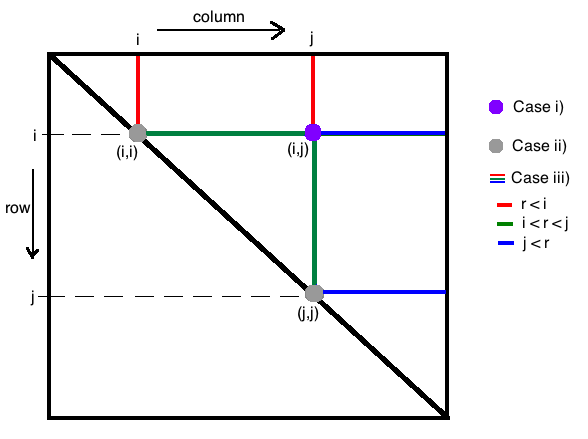
\includegraphics[scale=0.5]{Matrix.png}
\end{center}

We define a tolerance $tol=10^{-9}$ and perform rotations until the largest non-diagonal element is less than the tolerance. Since the matrix is symmetric we will perform rotations on the upper triangle of the matrix until it has converged.\\


For scenario i) we simply set the value of $A_{ij}'$ as 0. However, for scenario ii) we will look at the top left and bottom right elements in eq. 4 to gather equations to set the diagonal elements $A_{ii}'$ and $A_{jj}'$ . We have:
\begin{equation}
A_{ii}' = c^2 \cdot A_{ii} - 2cs\cdot A_{ij} + s^2\cdot A_{jj}
\end{equation}

From eq. 5 (because $A_{ij}'=0$) we can isolate $A_{jj}$ as\\
\begin{equation}
A_{jj} = A_{ii} - A_{ij}\frac{s^2-c^2}{cs}
\end{equation}
and since $c^2+s^2=1$ we simplify eq 14. as:
\begin{equation}
\begin{split}
A_{ii}' &= c^2 \cdot A_{ii} - 2cs\cdot A_{ij} + s^2\cdot A_{jj}\\
& = c^2 \cdot A_{ii} - 2cs\cdot A_{ij} + s^2 \left(A_{ii} - A_{ij}\frac{s^2-c^2}{cs}     \right)\\
& = (c^2 + s^2) \cdot A_{ii} - s\left(2c +  \frac{s^2-c^2}{c}      \right)A_{ij}\\
&= (c^2 + s^2) \cdot A_{ii} - \frac{s}{c}\left(2c^2 +  s^2-c^2      \right)A_{ij}\\
& = A_{ii} - \frac{s}{c}\left(c^2 +  s^2      \right)A_{ij}\\
& = A_{ii} - t\cdot A_{ij} 
\end{split}
\end{equation}
Similarly we have:\\
\begin{equation}
A_{jj}' = A_{jj} + t\cdot A_{ij}
\end{equation}



For scenario iii) we can look at top of eq 4. and note that if we consider an element $A_{rj}$ when we perform rotation around $A_{ij}$ that only the last two matrices will change the result since the first matrix changes rows i and j and does not have effect on row $r$. The last matrix changes columns i and j and therefore changes the resulting matrix. Multiplying through these matrices gives us the equations:
\begin{equation}
\bigg\{
  \begin{tabular}{cc}
$A_{ri}' = cA_{ri} - sA_{rj}$\\
$A_{rj}' = cA_{ri} + sA_{rj}$\\
  \end{tabular}
\end{equation}\\

Lets look at $A_{ri}'$ which can be represented as:
\begin{equation}
\begin{split}
A_{ri}' &= cA_{ri} - sA_{rj}\\
&= \left(1 - \frac{(1-c)(1+c)}{1+c} \right) A_{ri} - sA_{rj} \\
&= \left(1 - \frac{1-c^2}{1+c} \right) A_{ri} - sA_{rj} \\
&= \left(1 - \frac{s^2}{1+c} \right) A_{ri} - sA_{rj} \\
&= A_{ri}  - s \left(A_{rj} + \frac{s}{1+c} A_{ri} \right) \\
&= A_{ri}  - s \left(A_{rj} + \tau A_{ri} \right)  
\end{split}
\end{equation}

where 
\begin{equation}
\tau = \frac{s}{1+c}
\end{equation}

which has less roundoff error than eq. 18.\\

Similarly we have
\begin{equation}
A_{rj}' = A_{rj}  + s \left(A_{ri} - \tau A_{rj} \right) 
\end{equation}

\vspace{5mm}
To summarise we set values of elements in rows r and l and columns r and l as follows:
\begin{enumerate}[label=\roman*)]
  \item $A_{ij}=0$
\item $\bigg\{
  \begin{tabular}{cc}
$A_{ii}' = A_{ii} - t\cdot A_{ij}$  \\
$A_{jj}' = A_{jj} + t\cdot A_{ij}$ \\
  \end{tabular}$
\item $\bigg\{
  \begin{tabular}{cc}
$A_{ri}' = A_{ri}  - s \left(A_{rj} + \tau A_{ri} \right)$   \\
$A_{rj}' = A_{rj}  + s \left(A_{ri} - \tau A_{rj} \right)$   \\
  \end{tabular}$
\end{enumerate}

where
\[ s=t\cdot c, \hspace{5mm} t = \frac{sign(\theta)}{|\theta|+ \sqrt{1+\theta^2}}, \hspace{5mm} \tau = \frac{s}{1+c}, \hspace{5mm} \theta = \frac{A_{ii}-A_{jj}}{2A_{ij}}  \]







\end{document}







